W ramach projektu postanowiono poddać symulacji wytrzymałościowej również koła zębate.
    Z racji relatywnie dużych przełożeń poddano analizie wyłącznie parę kół zębatych wprowadzającą moment z bębna.
    Najbardziej obciążonymi rejonami w tym przypadku są współpracujące zęby.
    Oprócz tego występuje tutaj płaski stan naprężeń, co pozwala na uproszczenie symulacji do przypadku 2D (geometria na rysunku \ref{fig::geometria_plus_BC_przekladnia}). 
    Do obliczeń za materiał przyjęto stal konstrukcyjną.
    W symulacji zastosowano następujące warunki brzegowe:
    
    \begin{itemize}
    	\item Do wewnętrznej krawędzi większego koła zębatego przyłożono moment obrotowy o wartości 60 Nm (Obciążenie przenoszone z bębna). Oprócz tego nadano jej więz przemieszczeniowy, blokujący ruch w kierunku promieniowym.
    	\item Na powierzchniach styku zębów ustawiono warunek kontaktu z tarciem.
    	\item Wewnętrznej krawędzi mniejszego koła zębatego nadano więz przemieszczeniowy blokujący ruch w kierunku promieniowym oraz wymuszujący zadany obrót. Dzięki czemu uzyskano wyniki dla całego zakresu współpracy kół, dając pewność że znaleziono maksymalne naprężenia pojawiające się w obu elemenetach. 
    \end{itemize}
    

    \begin{figure}[th]
    	\centering
    	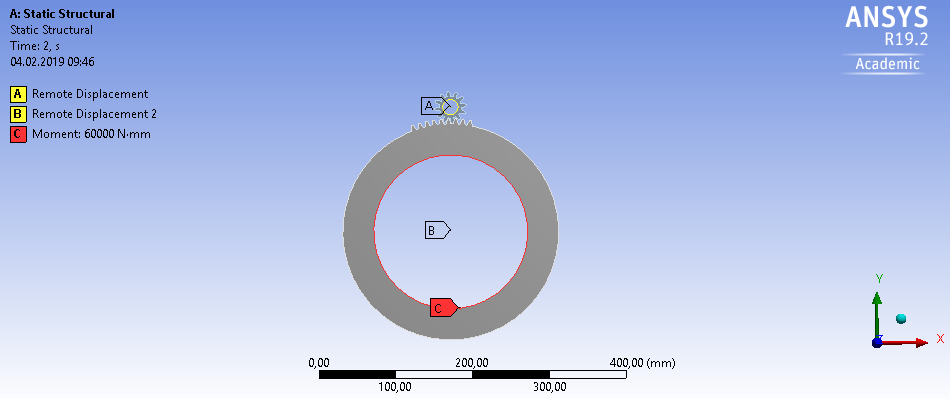
\includegraphics[width=0.9\linewidth]{Obliczenia/geometria_plus_BC_przekladnia}
    	\caption{Uproszczona geometria(usunięto zęby znajdujące się daleko od obszaru współpracy) użyta do wykonania symulacji.} 
    	\label{fig::geometria_plus_BC_przekladnia}
    \end{figure}

Znaczna część geometrii została podzielona siatką o dość dużych elementach, ponieważ nie przenoszą one znacznych obciążeń.
Jedynymi miejscami gdzie wykonano siatkę o dużej rozdzielczości z następującymi parametrami:
\begin{itemize}
	\item Na krawędziach styku nadano podział elementami o boku długości 0,027 mm. Dodatkowo obu krawędzi w głąb powierzchnii użyto funkcji inflation z pierwszą warstwą o grubości 0,01mm. Pozwoliło to uzyskać wysoką rozdzielczość na powierzchnii kontaktu obu ciał oraz zaraz pod nią, gdzie pojawiają się największe gradienty naprężeń.
	\item Reszta powierzchnii obu zębów wraz z ich niewielkim otoczeniem jest podzielona na elementy o boku 0,2mm.
	
\end{itemize}

\begin{figure}[bh]
	\centering
	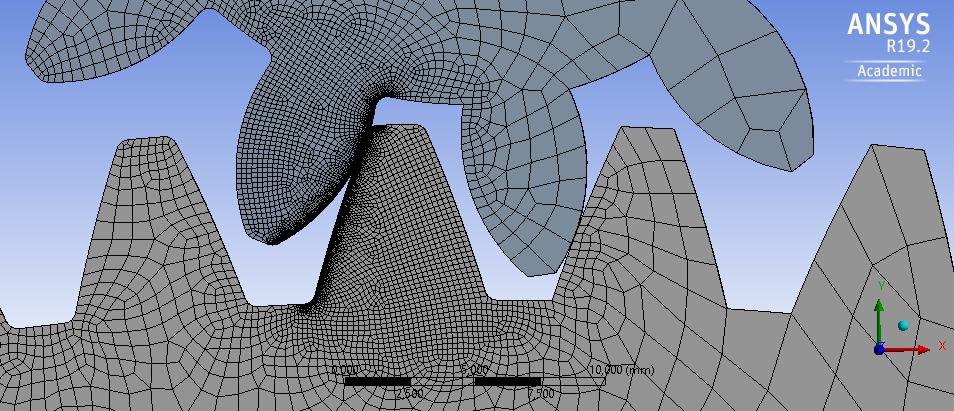
\includegraphics[width=0.9\linewidth]{Obliczenia/siatka_przekladnia}
	\caption{Siatka elementów skończonych użyta w opisywanej symulacji.} 
	\label{fig::geometria_plus_BC_przekladnia}
\end{figure}

Wyniki obliczeń przedstawiono na rysunku \ref{fig::geometria_plus_BC_przekladnia} w postaci naprężeń zredukowanych.
Jak widać naprężenia na znaczącym poziomie pojawiają tylko w pobliżu strefy kontaktu.
Z racji na ich wartość (259,97 MPa) zdecydowano, że koła zębate muszą być wykonane ze stali konstrukcyjnej C55 ulepszanej cieplnie do Re=500 MPa.
Zapewni to doraźny współczynnik bezpieczeństwa n=1.92.

\begin{figure}[th]
	\centering
	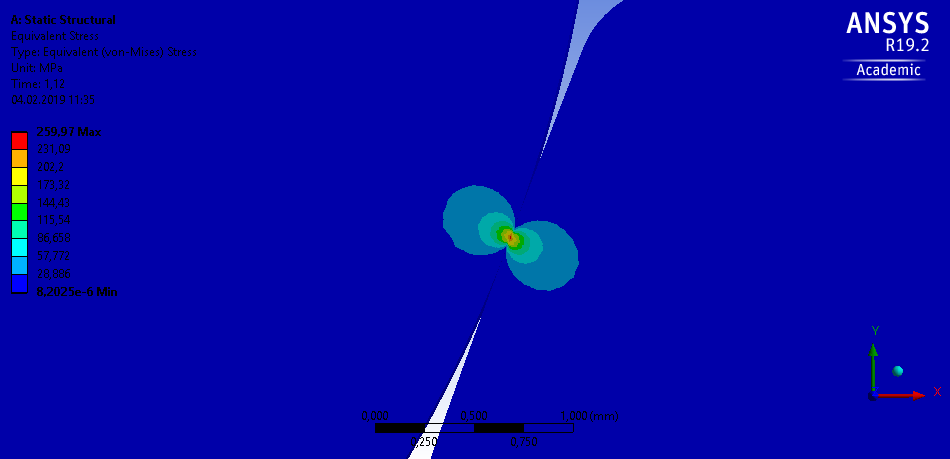
\includegraphics[width=0.9\linewidth]{Obliczenia/von_mises_stress_przekladnia}
	\caption{Naprężenia zredukowane(von Mises) dla ułożenia kół w którym występują najwyższe naprężenia zredukowane} 
	\label{fig::geometria_plus_BC_przekladnia}
\end{figure}